\subsubsection{GPUs in Computers}

Two main computer GPU setups are prominent today: \textit{integrated} graphical processing units (iGPU) and \textit{discrete} graphical processing units (dGPU), with the latter being most common both for consumer desktop computers as well as for scientific computing cluster nodes.
iGPUs are GPUs integrated onto the same die as a computer's CPU, where the two share the same physical \textit{Random Access Memory} (RAM) unit.

\begin{figure}[h!]\label{figure:gpu-system}
\begin{center}
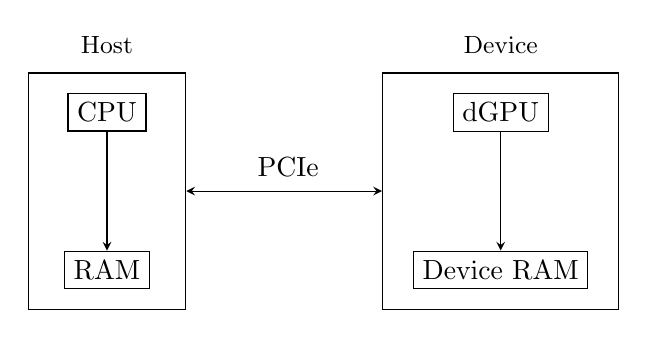
\begin{tikzpicture}

  \node at(0,2)[rectangle,draw](cpu){CPU};
  \node at(0,0)[rectangle,draw](cpuram){RAM};
  \node at(5,2)[rectangle,draw](gpu){dGPU};
  \node at(5,0)[rectangle,draw](gpuram){Device RAM};

  \node at(0,1)[rectangle,draw,minimum width=2cm,minimum height=3cm](host){};
  \node at(5,1)[rectangle,draw,minimum width=3cm,minimum height=3cm](device){};

  \draw [-stealth](cpu) -- (cpuram);
  \draw [-stealth](gpu) -- (gpuram);
  \draw [stealth-stealth](host) -- (device);

  \node at(2.3,1.3){\smaller PCIe};
  \node at(0,2.85){\small Host};
  \node at(5,2.85){\small Device};


\end{tikzpicture}
\caption{A typical CPU and dGPU setup.}
\end{center}
\end{figure}
